\chapter{Clustering e Topic Modelling, LLM e Prompting}

\section{Clustering Testuale con Embeddings}

\paragraph{La pipeline per il Clustering Testuale si articola in tre fasi:}

\begin{enumerate}
  \item Conversione dei documenti in vettori (\textit{embeddings}): su \fancyglitter{Hugging Face} è disponibile un modello pre-addestrato chiamato \textit{General Text Embeddings} (GTE). 
  \item Riduzione della dimensionalità degli embeddings: dato che gli embeddings hanno dimensioni elevate è necessario ridurli, per esempio con \fancyglitter{UMAP}. 
  \item Clustering dei vettori in gruppi significativi: per raggruppare documenti simili, si può usare \fancyglitter{HDBSCAN}.
\end{enumerate}

\nt {Successivamente c'è la fase di visualizzazione dei risultati (fig: \ref{fig:vis}), come visto in precedenza.}

\begin{figure}[h]
    \centering
    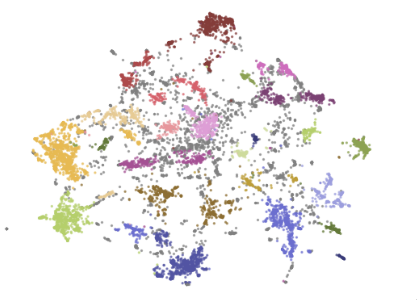
\includegraphics[scale=0.75]{04/visual.png}
    \caption{Visualizzazione dei dati.}
    \label{fig:vis}
\end{figure}

\subsection{BERTopic}

\dfn{BERTopic}{
  BERTopic è un framework moderno per il topic modelling. Si basa su:
  \begin{itemize}
    \item Una pipeline di clustering su embeddings testuali. 
    \item L'estrazione di parole salienti per ogni cluster attraverso \textit{class-based TF-IDF}.
  \end{itemize}
}

\paragraph{È possibile accedere alle informazioni dei topic estratti con i comandi:}

\begin{itemize}
  \item \texttt{topic\_model.get\_topic\_info()}. 
  \item \texttt{topic\_model.get\_topic()}.
\end{itemize}

\paragraph{Sono supportate diverse funzioni di interrogazione e visualizzazione:}

\begin{itemize}
  \item Ricerca di topic associati a una query. 
  \item Diagrammi interattivi: 
    \begin{itemize}
      \item \texttt{visualize\_documents()}. 
      \item \texttt{visualize\_barchart()}. 
      \item \texttt{visualize\_hierarchy()}. 
      \item \texttt{visualize\_heatmap()}.
    \end{itemize}
\end{itemize}












